\documentclass{article}
\usepackage{graphicx} % Required for inserting images
\usepackage[smartEllipses]{markdown}
\usepackage{geometry}

% Set the text width
\geometry{
    a4paper,
    left=2cm,
    right=2cm,
    top=2cm,
    bottom=2cm,
    marginparwidth=1.5cm,
    headheight=2cm
}

\usepackage{array}
\usepackage{makecell}

%Task and support template

%\begin{table}[htbp]
%    \centering
%    \begin{tabular}{|p{5cm}|p{10cm}|}
%        \hline
%        \multicolumn{2}{|c|}{\makecell[cl]{\textbf{Task:} \\
%        \textbf{Purpose:} \\
%        \textbf{Frequency:}}}\\
%        \hline
%        % Row 1
%        Sub task 1 & Example Solution 1 \\
%        \hline
%        % Row 2
%        ? & ? \\
%        \hline
%        % Row 3
%        ? & ? \\
%        \hline
%        % Row 4
%        ? & ? \\
%        \hline
%        \multicolumn{2}{|c|}{\makecell[cl]{\textbf{Variant:}}}\\
%        \hline
%        ? & ? \\
%        \hline
%    \end{tabular}
%    \caption{Example Table}
%    \label{tab:example}
%\end{table}



\title{Software Requirements Specification
Document\\
Cosy Koala IT}

\author{
  Vincent, Malzinskas\\
  \texttt{6474322}
  \and
  Aashim Lal, Memanaparambil Asokalal\\
  \texttt{103794571}
  \and
  Jordan, Zaz\\
  \texttt{6386601}
  \and
  Julian, Lai\\
  \texttt{103594920}
}

\date{March 2024}

\begin{document}

\maketitle
\newpage
\tableofcontents
\newpage


\section{Introduction}
This document contains the specifications for a operational information system (OIS) for the Cosy Koala restaurant in Hawthorn Vic. This document will outline the specifications, requirement and quality attributes of the operational information system

\subsection{Purpose}
The purpose of this document is to detail the functionalities and features of the OIS, aiming to streamline various restaurant operations as the business grows. From customer management and interactions to internal services and task management, the goal of this system is to allow the Cosy Koala to operate at a targeted customer patronage of 150 guests.

\subsection{Scope}
The OIS will facilitate the following high level tasks:
\begin{enumerate}
    \item Customer Management.
    \item Customer Interaction.
    \item Internal Services.
\end{enumerate}


\section{Project Overview}
The Cosy Koala currently sits 50 customers. It is making a physical expansion on premises to sit 150 customers. The current technical integration with operations is low. Taking orders from guest and interacting with the kitchen, and accounting is handled by hand.
The Cosy Koala has identified multiple ideas they would like to include in the OIS:
\begin{enumerate}
    \item The new system shall support reservations.
    \item The new system shall support taking orders from customers.
    \item The new system shall support information sharing with the Kitchen.
    \item The new system shall support creating invoices.
    \item The new system shall support creating receipts for customers.
    \item The new system shall support handling payments.
    \item The new system shall support basic statistics about ordered menu items.
    \item The new system shall support online availability of the menu.
    \item The new system shall support ordering from online take-away menus.
    \item The new system shall possibly support arranging delivery.
\end{enumerate}

\subsection{Domain Vocabulary}
\begin{enumerate}
    \item OIS : Operation Information System.
    \item FOH : Front of house.
    \item BOH : Back of house.
\end{enumerate}
\subsection{Pain Points}
\begin{enumerate}
    \item Customer information:
    \begin{enumerate}
        \item Managing 50+ customer orders.
        \item Taking onsite orders.
        \item Taking offsite orders.
        \item Collecting data on sales.
        \end{enumerate}
    \item Front to back of house interactions:
    \begin{enumerate}
        \item Organize orders.
        \item Make sure food is sent to correct customer.
    \end{enumerate}
    \item Administrative functions:
    \begin{enumerate}
        \item Gather customer data.
        \item Update website with marketing data.
        \item Analyse customer data.
        \item Provide offsite order and payment.
        \item Provide delivery.
    \end{enumerate}
\end{enumerate}


\subsection{Domain Entities}
\begin{enumerate}
    \item Meal
    \item Payments
    \item Customer
    \item Front of House Staff
    \item Seat
    \item Table
    \item Dining Room
    \item Receipts
    \item Sales Data
    \item Order
    \item Marketing Data, i.e. Menu lists, JPGs etc.
    \item Point of Sales
    \item Kitchen
\end{enumerate}


\subsection{Actors}
\begin{enumerate}
    \item Onsite Customer
    \item Offsite Customer
    \item Front of House Staff Member
    \item Back of House Staff Member
    \item Admin
    \item Website
    \item Delivery System
    \item EFTPOS or Banking System
\end{enumerate}

\subsection{Task - Brief}
\begin{enumerate}
    \item Take onsite customer order .
    \item Take offsite customer order.
    \item Take onsite customer payment.
    \item Take offsite customer payment.
    \item Create offsite customer receipt.
    \item Create onsite customer receipt.
    \item Communicate order with Kitchen.
    \item Seat customer.
    \item Drop food to customer.
    \item Deliver food to customer.
\end{enumerate}


\subsection{Project Goals \normalsize\textbf{Author: Vincent}}
\subsubsection{Primary Goals}
The primary Goal of Cosy Koala and the reason for releasing a tender for an OIS software provider is to be able to support a physical increase of guest from 50 to 150 in their restaurant.
\subsubsection{Secondary Goals}
\begin{enumerate}
    \item Support increased business through take-away.
    \item Support informed customers through their website.
    \item Support informed management about the customers purchases.
    \item Capture potential customers through their website.
\end{enumerate}
\subsubsection{Tertiary Goals}
Cosy Koala is interested in the possibility of supporting the arrangement of delivery.

\subsection{Assumptions \normalsize\textbf{Author: Vincent}}
A number of assumptions are made in relation to the implementation of this OIS is that manual scaling of operations are impossible. Whether that means no more staff will be available. Or whether staff will be expected to have other duties.

The system should model closely as possible to the current practices.


\clearpage

\section{Problem Domain}

\subsection{Data model \normalsize\textbf{Author: Vincent}}
\subsubsection{Domain model \normalsize\textbf{Author: Vincent}}
\begin{figure}[!ht]
    \centering
    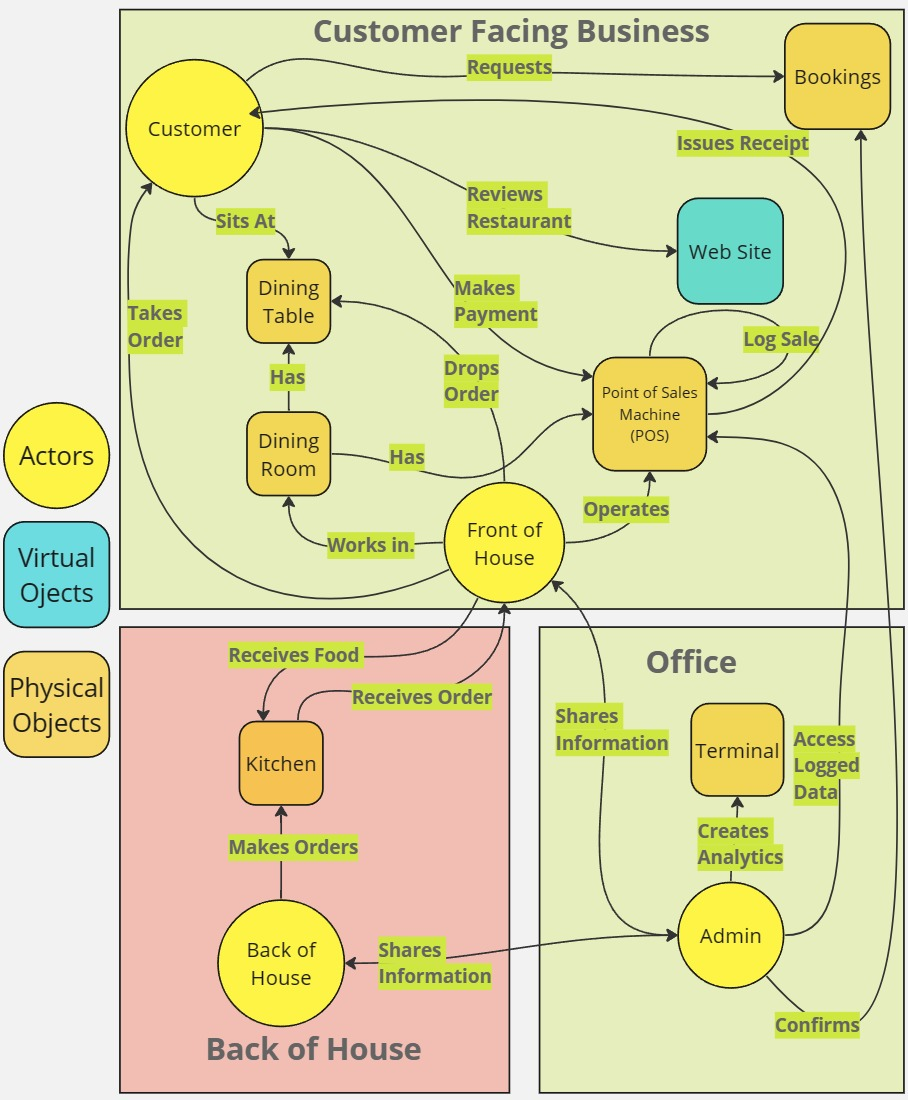
\includegraphics[width=15cm]{Domain_Model.jpg}
    \caption{Cosy Koala Domain Model}
    \label{fig:Domain_Model}
\end{figure}

\subsubsection{Entity Descriptions - Detailed}
\textbf{Meal:} To group together items for payment, delivery, or dropping at a table it would be helpful to place them into a unit of a meal. This way a meal can be paid for as one, or moved to a new table as one etc.

\textbf{Payments:} This will model the owed amounts for a meal, capable of of dividing payments based on a number of divisions, i.e. by item, by table, by room for functions. It will interact with receipts and and the Payment System (Actor).

\textbf{Customer:} This will model both the onsite and offsite customers, it will interact with bookings, tables, dining rooms, sales Data. It will contain customer specific data like meal, sales data.

\textbf{Front of House:} This will be a model for anyone interacting with customers capable of creating orders, bookings, taking payment and issuing receipts etc.

\textbf{Seat:} A customer can be assigned a seat to locate a meal or part of a meal to the correct customer.

\textbf{Table:} Contains seats and can be used for grouping meals into a larger single unit for booking or payment.

\textbf{Dining Room:} Containerizes and organizes customers orders i.e. If the restaurant has a multiple rooms this can be used to better locate customers for orders. It will contain tables which contain seats and customers.

\textbf{Receipts:} Will be a record for Sales data and Customers of a meal including its expense, items, time, location. Will be issues by the payment entity.

\textbf{Sales Data:} This is a aggregation of the Receipts data.

\textbf{Order:} (Onsite) Contains the meal order items, seat, table, dining room, that is ordered by a customer. \\(Offsite) Contains the meal order items, customer that is ordered by a customer.

\textbf{Marketing Data:} This will be the data that can be sent to the Website (Actor) in order to update the website.

\textbf{Point of Sales Machine:} Facilitates payment transactions. Issues receipts. Logs sales data. Is operated be a front of house staff member. Interacts with the payment entity and the payment system (Actor)

\textbf{Kitchen:} Containerizes and organizes customers food order for pick up by front of house.



\subsection{Actors Descriptions - Detailed}

\textbf{Onsite Customer:} Is a person dining on food or beverages prepared by Cosy Koala. This is done on site in a dining room at a table. .

\textbf{Offsite Customer:} Is a person dining on food or beverages prepared by Cosy Koala. This is done off site at any location other than Cosy Koala dining rooms.

\textbf{Front of House:} This is a staff member who has direct contact with the customer. They take orders from customers. Take orders to the Kitchen. Bring customers their food. They are responsible for maintaining the orders integrity (Making sure the customer gets what they pay for). The take customer transactions. Communicate with Admin.

\textbf{Back of House:} Prepare the customers food order. Responsible for making sure front of house receive the food order with correct information i.e. order number etc. Communicate with Admin.

\textbf{Website:} Displays the restaurant information for customers.

\textbf{Admin:} Get the logged data from the Point of Sales Machine.
Generate analytics from the Sales data.
Web Site: Display general information about the restaurant.

\textbf{EFTPOS or Banking System:} This is the outside system that will have to interact with the POS entity in order to facilitate payments.

\textbf{Delivery System:} This the outside system that facilitates delivery, like Uber, or menulog etc.


\clearpage
\subsection{Workflows \normalsize\textbf{Author: Vincent}}

\begin{table}[htbp]
    \centering
    \begin{tabular}{|p{5cm}|p{10cm}|}
        \hline
        \multicolumn{2}{|c|}{\makecell[cl]{\textbf{Task: Administrate the restaurant} \\
        \textbf{Actor: Admin} \\
        \textbf{Purpose:} To manage the technical administration tasks so that everything from bookings\\
        to invoices are completed in a timely correct manner.}}\\
        \hline
        % Row 1
        Sub task  & Example Solution  \\
        \hline
        % Row 2
        1. Review past data, including sales, costs, etc, particular attention is paid to the past day of service.
        
        \textbf{Problem:} Records are not accurate. & Communicate directly with staff from the previous day about the data generated. Automate data entry. \\
        \hline
        % Row 3
        2. Update restaurant bookings, and communicate with customers. 
        
        \textbf{Problem:} Bookings are unavailable for guest. & Communicate with the guest about an alternative date to book. Make the available dates and services on a given date accessible to customers. \\
        \hline
        % Row 4
        3. Communicate and inform the FOH and BOH staff about upcoming customer demands, bookings and general workload. 
        
        \textbf{Problem:} The bookings are changing rapidly or give short notice & Auto update FOH and BOH staff about bookings etc. \\
        \hline
    \end{tabular}
    \caption{Workflow: 1}
    \label{tab:example_wf_1}
\end{table}

\clearpage
\begin{table}[htbp]
    \centering
    \begin{tabular}{|p{5cm}|p{10cm}|}
        \hline
        \multicolumn{2}{|c|}{\makecell[cl]{\textbf{Task: Prepare the kitchen} \\
        \textbf{Actor: Back of House} \\
        \textbf{Purpose:} To prepare enough food or drink for the upcoming guest, planning at the service, \\day and week level is appropriate.}}\\
        \hline
        % Row 1
        Sub task  & Example Solution  \\
        \hline
        % Row 2
        1. Review bookings for today and tomorrow in close detail as well as a week ahead in brief detail. 
        
        \textbf{Problem:} Records are not accurate. Bookings have change but kitchen doesn't know. & Automate directly live data to the kitchen. \\
        \hline
        % Row 3
        2. Receive orders and cook food. 
        
        \textbf{Problem:} Orders are not accurate to items and customers & Deliver orders to kitchen directly from order entry at POS machine, - no hand written dockets. \\
        \hline
        % Row 4
        3. Order needed food for upcoming bookings. 
        
        \textbf{Problem:} Bookings have not been updated. & Automate directly live data to the kitchen. \\
        \hline
    \end{tabular}
    \caption{Workflow: 2}
    \label{tab:example_wf_2}
\end{table}


\clearpage
\begin{table}[htbp]
    \centering
    \begin{tabular}{|p{5cm}|p{10cm}|}
        \hline
        \multicolumn{2}{|c|}{\makecell[cl]{\textbf{Task: Receive and dine guests} \\
        \textbf{Actor: Front of House} \\
        \textbf{Purpose:} To prepare the room/s fro upcoming guest, planning at the service\\ and day is appropriate.}}\\
        \hline
        % Row 1
        Sub task  & Example Solution  \\
        \hline
        % Row 2
        1. Review bookings for today in close detail. 
        
        \textbf{Problem:} Records are not accurate. Bookings have change but front of house staff don't know. & Automate directly live data to the front of house staff. \\
        \hline
        % Row 3
        2. Set tables and places for bookings and expected walk ins. 
        
        \textbf{Problem:} Bookings have change but front of house staff don't know. & Automate directly live data to the front of house staff. \\
        \hline
        % Row 4
        3. Receive guest/s. Take to booked seating.
        
        \textbf{Problem:} Guest/s has not booked & Find the available tables and seats.\\
        \hline
        4. Take orders from guests. 
        
        \textbf{Problem:} The guest changes meal order, guest changes table or seat, guests leave, more guest come. & Have flexible table and meal placement that can be altered.\\
        \hline
        5. Take payment. 
        
        \textbf{Problem: } Payment is to be split by meal, item, guest, table or some other way. & Make a flexible payment option.\\
        \hline
    \end{tabular}
    \caption{Workflow: 3}
    \label{tab:example_wf_3}
\end{table}



\clearpage
\subsection{Tasks}

\subsection{Complete Payment transaction onsite.}
\begin{table}[htbp]
    \centering
    \begin{tabular}{|p{5cm}|p{10cm}|}
        \hline
        \multicolumn{2}{|c|}{\makecell[cl]{\textbf{Task:} Complete Payment transaction onsite. \\
        \textbf{Purpose:} Take the money owed to the restaurant after a sale of a food or drink and issue receipt.\\
        \textbf{Frequency:} Up to 150 times a breakfast, lunch or dinner service.}}\\
        \hline
        % Row 1
        \textbf{Sub task} & \textbf{Example Solution} \\
        \hline
        % Row 2
        Locate the meal in system. & Enter the table number, and dining room name in order to find the meal. \\
        \hline
        % Row 3
        Inform customer of details of meal, price etc. & The GUI can display relevant meal information. \\
        \hline
        % Row 4
        Initiate payment system. & FoH Staff member can send the price of the meal to the EFTPOS machine. \\
        \hline
        % Row 5
        Display whether the payment was successful. & The GUI can display to the customer and the staff member whether payment was successful. \\
        \hline
        % Row 6
        Offer to print receipt. & The GUI could display an option for the FoH or Customer to select to print a receipt. \\
        \hline
        Print receipt & System send information to printer, possibly by network. \\
        \hline
        Move transaction to new state - payed & The system can validate the transaction was successful and move the meal to a payed/cleared data storage. \\
        \hline
        \multicolumn{2}{|c|}{\makecell[cl]{\textbf{Variant:}}}\\
        \hline
        Customer only wants to pay for their meal and a table with multiple people & System should allow the FoH to select items from a meal for individual payment. \\
        \hline
    \end{tabular}
    \caption{Taking Payment}
    \label{tab:Complete Payment transaction onsite.}
\end{table}

\clearpage
\subsection{Take a booking}
\begin{table}[htbp]
    \centering
    \begin{tabular}{|p{5cm}|p{10cm}|}
        \hline
        \multicolumn{2}{|c|}{\makecell[cl]{\textbf{Task:} Take a customers booking. \\
        \textbf{Purpose:} To pre-allocate a customer to a table in order to make sure the customer can dine when arriving. \\
        \textbf{Frequency:} Up to 150 time a service, 3 services a day.}}\\
        \hline
        % Row 1
        \textbf{Sub task} & \textbf{Example Solution} \\
        \hline
        % Row 2
        Receive customers correspondance - email, phone call & Each day the admin will check the restaurant email and collect any bookings that have been sent.  \\
        \hline
        % Row 3
        For each booking review availability. & If some one wants to book a table for 4 at 8pm on Friday, the admin will first check if there is space for a table of 4 at that date and time. \\
        \hline
        % Row 4
        Enter booking into record. & The admin will make a recording of the booking so that the resources cannot be double booked. \\
        \hline
        Inform the Front of house staff & The admin will transfer the bookings for today to a sheet for the front of house to organise the dining room to host. \\
        \hline
        Return confirmation correspondence to the customer & The admin will send a return email with the confirmation details.\\
        \hline
        \multicolumn{2}{|c|}{\makecell[cl]{\textbf{Variant:}}}\\
        \hline
        The Admin receives a phone call. & This booking will need to be reviewed on the spot in order to make confirmation. \\
        \hline
        The booking is made on short notice & After the bookings and confirmation have already been made for the day. A new booking comes in. The admin will need to directly confirm and inform front of house to accommodate the booking. \\
        \hline
        The booking cannot be made. & The admin must reject the booking and offer a possible alternative.\\
        \hline
    \end{tabular}
    \caption{Take a booking}
    \label{tab:Take a booking}
\end{table}

\clearpage
\subsection{Take a tables order}
\begin{table}[htbp]
    \centering
    \begin{tabular}{|p{5cm}|p{10cm}|}
        \hline
        \multicolumn{2}{|c|}{\makecell[cl]{\textbf{Task:} \\
        \textbf{Purpose:} \\
        \textbf{Frequency:}}}\\
        \hline
        % Row 1
        Sub task 1 & Example Solution 1 \\
        \hline
        % Row 2
        ? & ? \\
        \hline
        % Row 3
        ? & ? \\
        \hline
        % Row 4
        ? & ? \\
        \hline
        \multicolumn{2}{|c|}{\makecell[cl]{\textbf{Variant:}}}\\
        \hline
        ? & ? \\
        \hline
    \end{tabular}
    \caption{Take a tables order}
    \label{tab:Take a tables order}
\end{table}

\clearpage
\subsection{Cook Food}
\begin{table}[htbp]
    \centering
    \begin{tabular}{|p{5cm}|p{10cm}|}
        \hline
        \multicolumn{2}{|c|}{\makecell[cl]{\textbf{Task:} \\
        \textbf{Purpose:} \\
        \textbf{Frequency:}}}\\
        \hline
        % Row 1
        Sub task 1 & Example Solution 1 \\
        \hline
        % Row 2
        ? & ? \\
        \hline
        % Row 3
        ? & ? \\
        \hline
        % Row 4
        ? & ? \\
        \hline
        \multicolumn{2}{|c|}{\makecell[cl]{\textbf{Variant:}}}\\
        \hline
        ? & ? \\
        \hline
    \end{tabular}
    \caption{Cook Food}
    \label{tab:Cook Food}
\end{table}

\clearpage
\subsection{Create Analytics}
\begin{table}[htbp]
    \centering
    \begin{tabular}{|p{5cm}|p{10cm}|}
        \hline
        \multicolumn{2}{|c|}{\makecell[cl]{\textbf{Task:} \\
        \textbf{Purpose:} \\
        \textbf{Frequency:}}}\\
        \hline
        % Row 1
        Sub task 1 & Example Solution 1 \\
        \hline
        % Row 2
        ? & ? \\
        \hline
        % Row 3
        ? & ? \\
        \hline
        % Row 4
        ? & ? \\
        \hline
        \multicolumn{2}{|c|}{\makecell[cl]{\textbf{Variant:}}}\\
        \hline
        ? & ? \\
        \hline
    \end{tabular}
    \caption{Create Analytics}
    \label{tab:Create Analytics}
\end{table}

\clearpage
\subsection{Update Website}
\begin{table}[htbp]
    \centering
    \begin{tabular}{|p{5cm}|p{10cm}|}
        \hline
        \multicolumn{2}{|c|}{\makecell[cl]{\textbf{Task:} \\
        \textbf{Purpose:} \\
        \textbf{Frequency:}}}\\
        \hline
        % Row 1
        Sub task 1 & Example Solution 1 \\
        \hline
        % Row 2
        ? & ? \\
        \hline
        % Row 3
        ? & ? \\
        \hline
        % Row 4
        ? & ? \\
        \hline
        \multicolumn{2}{|c|}{\makecell[cl]{\textbf{Variant:}}}\\
        \hline
        ? & ? \\
        \hline
    \end{tabular}
    \caption{Update Website}
    \label{tab:Update Website}
\end{table}

\clearpage
\subsection{Drops food to table}
\begin{table}[htbp]
    \centering
    \begin{tabular}{|p{5cm}|p{10cm}|}
        \hline
        \multicolumn{2}{|c|}{\makecell[cl]{\textbf{Task:} \\
        \textbf{Purpose:} \\
        \textbf{Frequency:}}}\\
        \hline
        % Row 1
        Sub task 1 & Example Solution 1 \\
        \hline
        % Row 2
        ? & ? \\
        \hline
        % Row 3
        ? & ? \\
        \hline
        % Row 4
        ? & ? \\
        \hline
        \multicolumn{2}{|c|}{\makecell[cl]{\textbf{Variant:}}}\\
        \hline
        ? & ? \\
        \hline
    \end{tabular}
    \caption{Drops food to table}
    \label{tab:Drops food to table}
\end{table}

\clearpage
\subsection{Share information Admin-Front of house, Admin-Back of house.}
\begin{table}[htbp]
    \centering
    \begin{tabular}{|p{5cm}|p{10cm}|}
        \hline
        \multicolumn{2}{|c|}{\makecell[cl]{\textbf{Task:} \\
        \textbf{Purpose:} \\
        \textbf{Frequency:}}}\\
        \hline
        % Row 1
        Sub task 1 & Example Solution 1 \\
        \hline
        % Row 2
        ? & ? \\
        \hline
        % Row 3
        ? & ? \\
        \hline
        % Row 4
        ? & ? \\
        \hline
        \multicolumn{2}{|c|}{\makecell[cl]{\textbf{Variant:}}}\\
        \hline
        ? & ? \\
        \hline
    \end{tabular}
    \caption{Admin communication}
    \label{tab:Admin communication}
\end{table}

\clearpage
\subsection{}
\begin{table}[htbp]
    \centering
    \begin{tabular}{|p{5cm}|p{10cm}|}
        \hline
        \multicolumn{2}{|c|}{\makecell[cl]{\textbf{Task:} \\
        \textbf{Purpose:} \\
        \textbf{Frequency:}}}\\
        \hline
        % Row 1
        Sub task 1 & Example Solution 1 \\
        \hline
        % Row 2
        ? & ? \\
        \hline
        % Row 3
        ? & ? \\
        \hline
        % Row 4
        ? & ? \\
        \hline
        \multicolumn{2}{|c|}{\makecell[cl]{\textbf{Variant:}}}\\
        \hline
        ? & ? \\
        \hline
    \end{tabular}
    \caption{Example Table}
    \label{tab:example}
\end{table}






\subsection{Functional Requirements and Task Descriptions}
\begin{figure}[!ht]
    \centering
    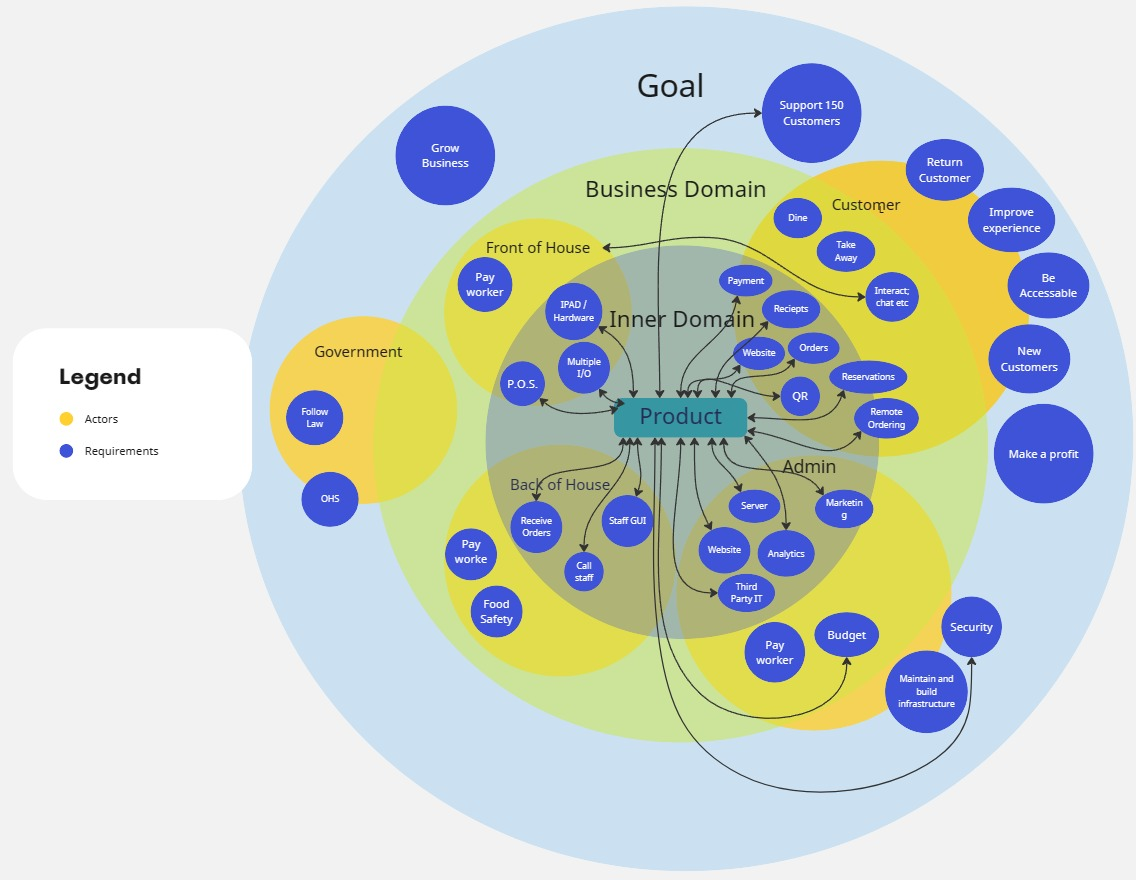
\includegraphics[width=15cm]{Domain_product_diagram.jpg}
    \caption{Cosy Koala Domain Requirements}
    \label{fig:Domain_Product}
\end{figure}

\section{Quality Attributes of System}
\section{Other Requirements}
\section{Validation of Requirements}
\section{Possible Solutions}


\end{document}
